% !TeX root =../../main.tex

\chapter{Introduction} \label{ch:introduction}


\section{Motivations and Challenges}
Software systems usually suffer from various kinds of vulnerabilities and weakness. These vulnerabilities can cause huge catastrophes from financial property loss to massive personnel casualty. For example, \emph{Heartbleed}(CVE-2014-0160)~\cite{heartbleed} is a critical vulnerability caused by an implementation defect in the widely used OpenSSL cryptographic software library which can compromise the integrity of communications across the entire Web. Further, it is reported that this may also affect the internal networks of enterprise in the coming years due to the fact that most enterprises do not have a good handle on the SSL encrypted services. Other software weakness may lead to more direct tragedies which lead to deaths. For example, the aircraft accident of Ethiopian Airlines Flight 302 in the late 2018 is high likely due to the improper functionality of the Maneuvering Characteristics Augmentation System (MCAS) from Boeing 737 Max~\cite{boeing_Ethiopian}. 153 lives were lost during this accident, including 149 passengers and 8 crew. Ironically, MCAS is designed to keep the balance of the airplane. The same Boeing 737 Max jet led to totally 189 people's death during Lion Air Flight 610 in 2019, which probably results from the functionality of MCAS.

One interesting phenomenon needs to pay attention to is that it is usually a long time from \emph{the point that the vulnerability was introduced} to \emph{the point when the corresponding software was fully upgraded to the patched versions}. According to ``Vulnerability Review 2018 -- Global Trends''~\cite{vul_flexera18}, there are 86\% vulnerabilities had a patch available on the day of disclosure in 2017, while in 2016 this percentage is 81\%. It is worth noting that some vendors choose to issue major product releases only. For the Heartbleed case, it is also interesting that this vulnerability was introduced in 2012 while was not discovered until 2 years later in 2014. Worse still, it also remains unknown when all the mainstream services will be upgraded to get grid of this vulnerability eventually. For the Boing 737 Max case, it is even unclear to the public whether there is a solution for the remedy at all, despite the fact that its first flight was January, 2016, which has passed 3 years.

In order to avoid the damages brought by the software defects, it is favorable to disclose these vulnerabilities as early as possible and fix them immediately. The most widely applied approaches are \emph{dynamic testing} and \emph{verification}. For testing, we feed the software with multiple test corpus, which can be a variety of test files, a sequence of the events, etc. This checks the different functionalities of the program under test by considering different application scenarios. It can detect the weakness when it finds a violation with the given test suite; if no error reports, however, it does not mean there are no vulnerabilities inside. On the other hand, verification usually guarantees that the underlying software systems are free of certain considered vulnerabilities. Due to its complexity nature, the programs or the systems that are verified are usually abstracted in an intermediate representation and the focus is a relative higher level security guarantee.

\section{Main Work}

This work aims to secure the software systems with both \emph{testing} and \emph{verification} approaches. Fig.~\ref{fig:works} depicts the main work of the thesis and their relations.

For testing, we apply the grey-box fuzzing approaches to reveal those \emph{implementation induced vulnerabilities}. We firstly build a grey-box fuzzing framework called \emph{Fuzzing Orchestration Toolkit}, or \FOT by short. This framework aims to be \emph{versatile}, \emph{configurable}, and \emph{extensible}. It is versatile since it has integrated and will integrate various grey-box fuzzing techniques~\cite{Bohme:2016:CGF,Bohme:2017:DGF,redqueen,CollAFL,Angora,fuzz_survey}. It is configurable in that it provides several builtin strategies which allow easy customization for the fuzzing procedure. It is also extensible in that it provides fruitful interfaces for easy integration with new techniques. We also apply two novel extensions to \FOT from two aspects. In order to guide the fuzzing procedure to \emph{certain specific program locations}, we propose \dFOT; this can be applied to scenarios such as patching testing, crash reproduction, etc. We pointed out four key properties that are considered important to the guidance: the robust directedness mechanism, the lightweight yet effective integration with static analysis, the optimized seed prioritization and scheduling strategies, as well as the adaptive strategies across fuzzing states. In order to improve the efficiency of fuzzing multi-threaded programs, we propose \mtfuzz, which utilizes the thread-aware analyses to increase the quality of the generated seeds. \mtfuzz provides the thread-interleaving feedback by providing a novel stratified exploration oriented instrumentation, together with the threading context information and the thread scheduling intervention that diversifies the actual interleaving.

Although fuzzing can reveal the implementation specific vulnerabilities, it usually lacks the insight of the higher level design vulnerabilities. For example, although it is possible for fuzz testing to discover multiple crashes in the libraries and Android runtime, it usually cannot reveal certain categories of various security issues regarding privacy at the application framework level and the applications built on top of it~\cite{Enck:2009:UAS:1512148.1512324,Ernst:2014}. In fact, it is almost impossible for testing to detect certain security issues in Android due to its designing flaw~\cite{url:android-flaw}. In order to secure the higher level defects such as the information leakage in Android system, we propose a security type system in order to rigorously certify that the underlying system is free of information leakage. The novelty of the proposed security type system is that we designed a type merging operator that allows for permission-dependent security types. We proved the soundness of the type system in terms of \emph{non-interference}, in which we formally assure no information leakage in the system as long as the security type checking is passed. We also provided a set of type inference rules that are guaranteed to be decidable in finite numbers of steps. In addition, we implemented a prototype of the type system which can type check the information leakage issues in Android.

With these two applied approaches, we aim to provide a comprehensive solution to securing the various software systems such as Linux or Android.

\begin{figure}[ht]
	\begin{center}
		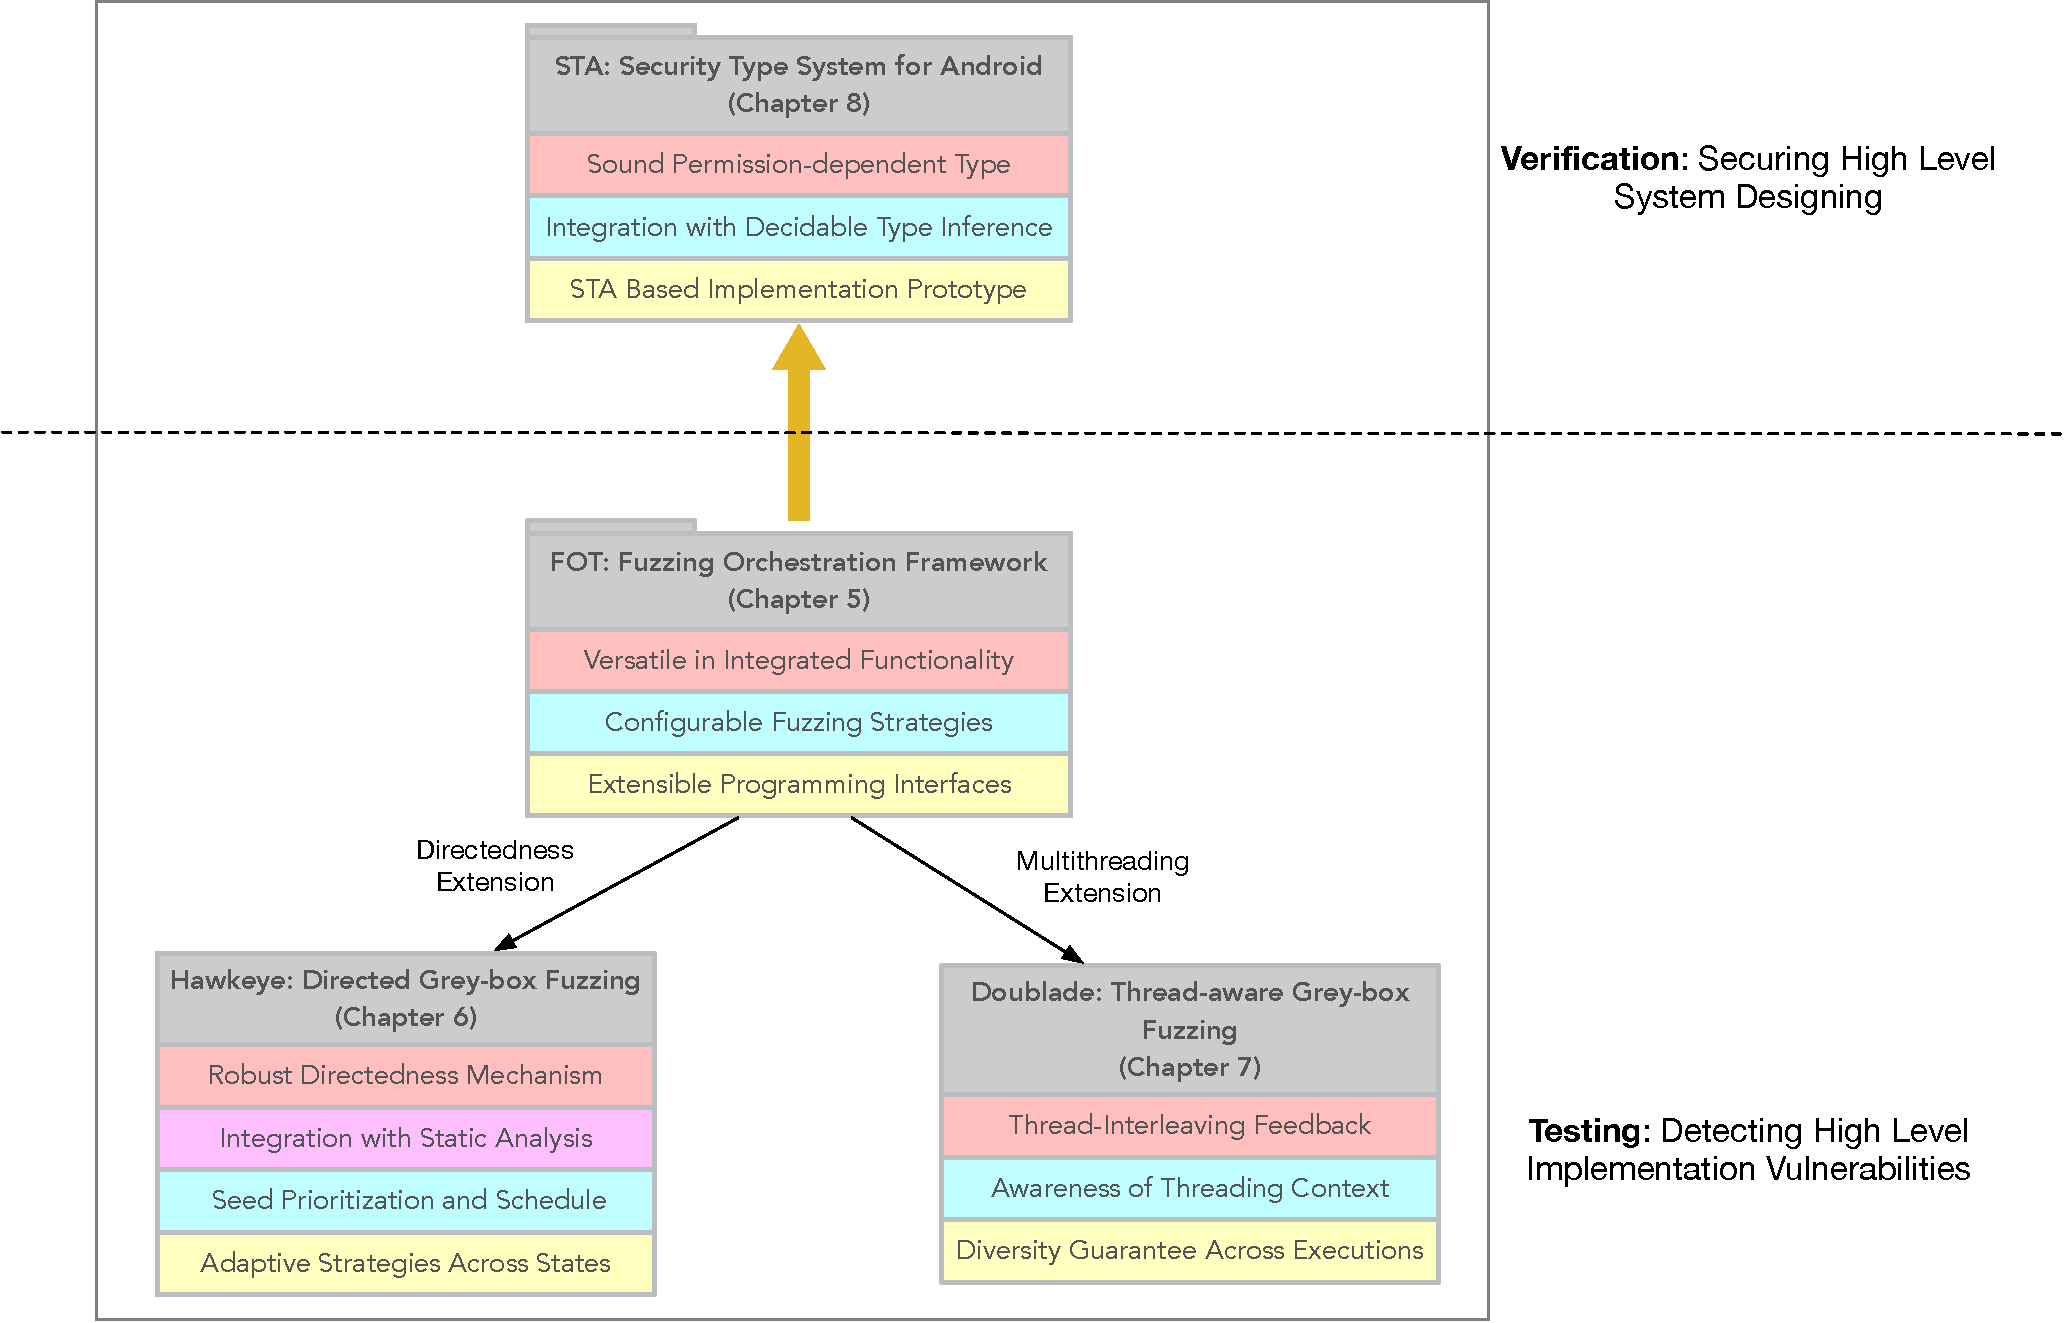
\includegraphics[width=0.98\textwidth]{res/contributions}
		\caption{Main Work of the Thesis and the Relations}
		\label{fig:works}
	\end{center}
\end{figure}

\section{Contributions of the Thesis}
The contributions of the thesis is as follows:
\begin{enumerate}
	\item We provided a grey-box fuzzing framework, \FOT, that is versatile in its configurability and extensibility.
	\item We proposed a principled directed grey-box fuzzing technique \dFOT to allow for fuzzing on specific program targets and implemented it on top of \FOT.
	\item We proposed a thread-aware fuzzing technique, \mtfuzz, which significantly improved the effectiveness of fuzzing on multi-threaded programs.
	\item We provided a permission-dependent type system that can precisely enforce the access control based on the permission authentication, provided the soundness, the decidability of type inference, and implemented a prototype for securing Android system.
\end{enumerate}


\section{List of Materials Related to the Thesis}
\begin{enumerate}
	\item \myname, Yuekang Li, Bihuan Chen, Yinxing Xue, Yang Liu, ``FOT: A Versatile, Configurable, Extensible Fuzzing Framework'', ESEC/FSE '18, Proceedings of the 2018 26th ACM Joint Meeting on European Software Engineering Conference and Symposium on the Foundations of Software Engineering, Pages 867-870, \url{http://doi.acm.org/10.1145/3236024.3264593}, DOI: 10.1145/3236024.3264593.
	\item \myname, Yinxing Xue, Yuekang Li, Bihuan Chen, Xiaofei Xie, Xiuheng Wu, Yang Liu, ``Hawkeye: Towards a Desired Directed Grey-box Fuzzer'', CCS'18, Proceedings of the 2018 ACM SIGSAC Conference on Computer and Communications Security, Pages 2095-2108, \url{http://doi.acm.org/10.1145/3243734.3243849}, DOI: 10.1145/3243734.3243849.
	\item \myname, Shengjian Guo, Yinxing Xue, Yulei Sui, Cen Zhang, Yuekang Li, Haijun Wang, Yang Liu, ``Doublade: Enhancing Grey-box Fuzzing for Multithreaded Programs with Thread-aware Analysis'', submitted.
	\item \myname, Alwen Tiu, Zhiwu Xu, Yang Liu, ``A Permission-Dependent Type System for Secure Information Flow Analysis'', 2018 IEEE 31st Computer Security Foundations Symposium (CSF'18), Oxford, 2018, pp. 218-232. \url{https://doi.org/10.1109/CSF.2018.00023}, DOI: 10.1109/CSF.2018.00023. A technical report is available at \url{https://arxiv.org/abs/1709.09623}.
\end{enumerate}

\section{Outline of the Thesis}

The rest of this thesis is organized as follows.

Chapter~\ref{ch:related} describes the related work of this thesis. Chapter~\ref{ch:fot} describes the recent progress of fuzzing and several aspects of challenges, and introduces our grey-box fuzzing framework, \FOT, which aims to solve these issues. Chapter~\ref{ch:dfot} explains our directed grey-box fuzzer \dFOT built on top of \FOT; \dFOT is our attempt to guide the fuzzing process to specific program targets. Chapter~\ref{ch:mtfuzz} describes \mtfuzz based on \FOT, which aims to enhance the effectiveness of fuzzing on multithreaded programs. Chapter~\ref{ch:sta} describes our attempt to secure software systems based on verification, which applies a permission-dependent type system to enforce the non-interference property that prevents the information leakage in an Android-like system. Chapter~\ref{ch:discuss} discusses my reflection on the testing and verification based techniques. Chapter~\ref{ch:conclusion} concludes this thesis and describes the possible future work.